\documentclass[11pt,a4paper]{article}
\usepackage[utf8]{inputenc}
\usepackage[T1]{fontenc}
\usepackage[spanish]{babel}
\usepackage[margin=2cm]{geometry}
\usepackage{graphicx,url}
\pagestyle{empty}

\begin{document}

\begin{center}
{\Large\bfseries Universidad Técnica Estatal de Quevedo}\\
Facultad de Ciencias de la Computación --- Carrera de Software
\end{center}

\noindent\textbf{Apellidos y nombres:} Sánchez Centeno Roselyn Andreina\\
\textbf{Asignatura:} Ingeniería de Requerimientos (ISR-401)\\
\textbf{Nivel y paralelo:} 4.º nivel, Paralelo B\\
\textbf{Tarea:} EV-PRAC-01, Evaluación de la Unidad I\\
\textbf{Fecha de la sesión:} 18 de noviembre de 2026\\
\textbf{Fecha límite de entrega:} 18 de noviembre de 2026, 23:59\\
\textbf{URL del repositorio:}\\
{\footnotesize\url{https://github.com/Roselyn15/EV-PRAC-01_RoselynSanchez_4toB}}

\vspace{0.5cm}
\begin{center}
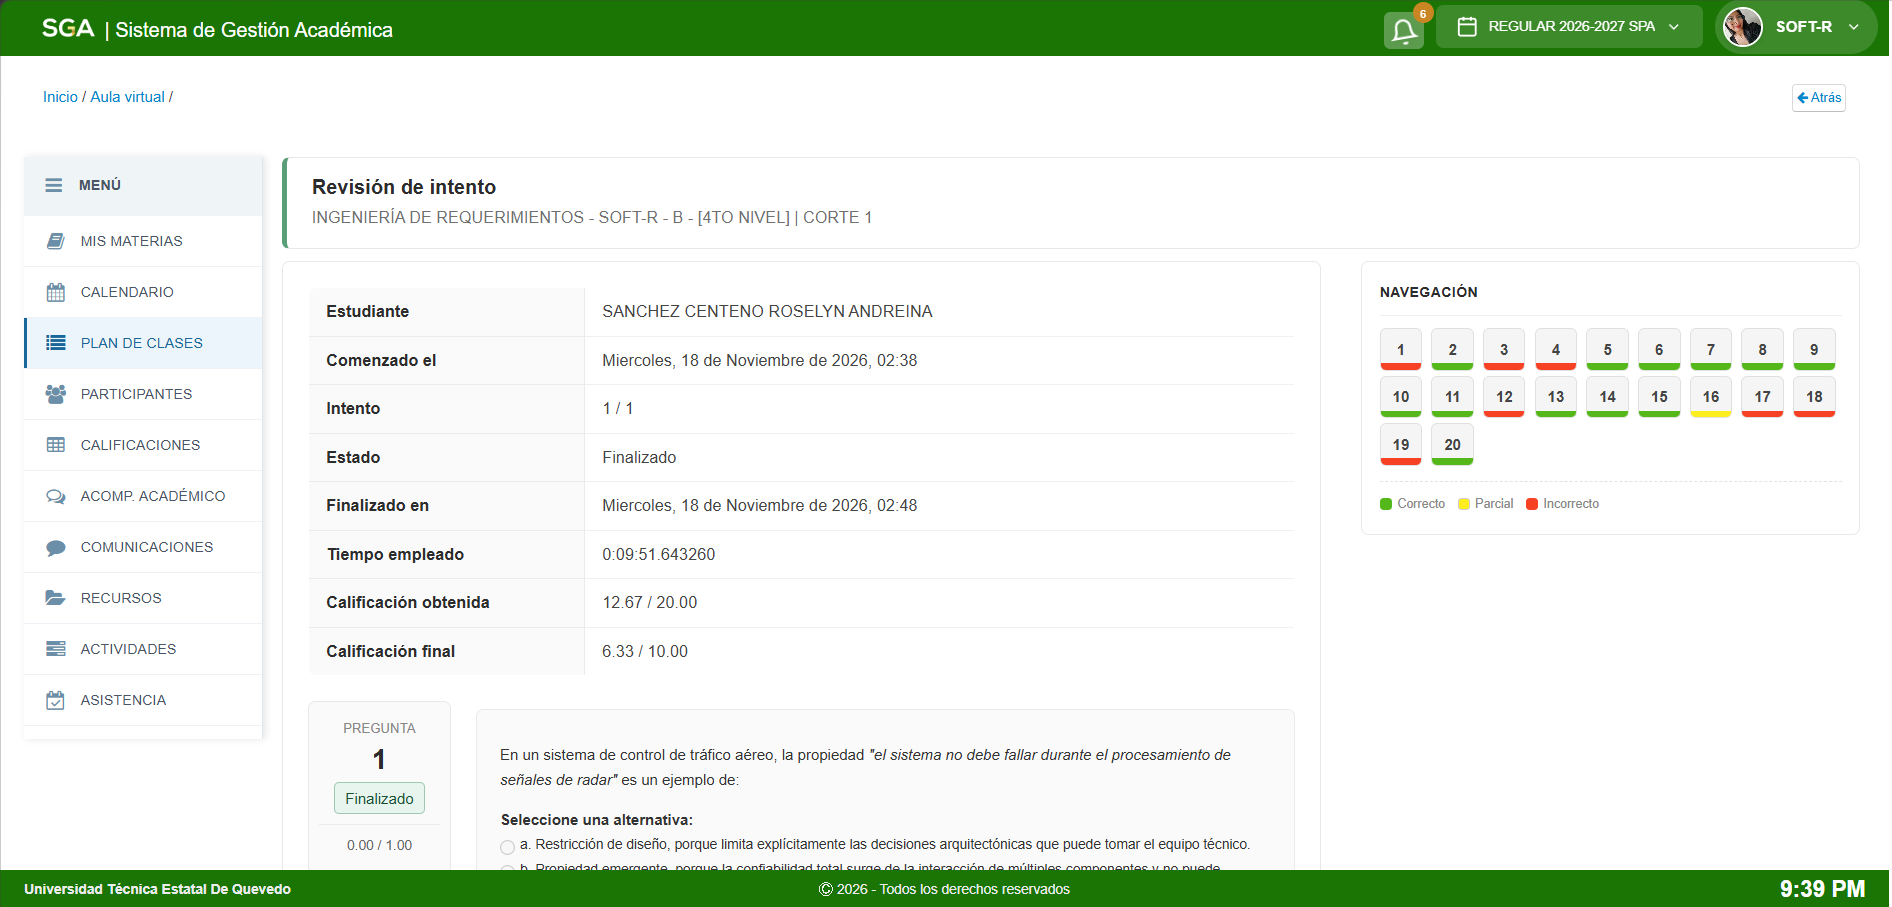
\includegraphics[width=\textwidth,height=15cm,keepaspectratio]{captura_intentodelcuestionario.png}
\end{center}

\end{document}
